\documentclass{article}

\usepackage{latexsym}
\usepackage{bbm}
\usepackage[small,bf]{caption2}
\usepackage{graphics}
\usepackage{epsfig}
\usepackage{amsmath,amssymb,amsthm,amsfonts}
\usepackage{url}
\usepackage{hyperref}
\usepackage{enumerate}
\usepackage{xspace}

\usepackage{tikz}
\usetikzlibrary{shapes.geometric, arrows}

%% Page size
\setlength{\oddsidemargin}{0pt}
\setlength{\evensidemargin}{0pt}
\setlength{\textwidth}{6.5in}
\setlength{\topmargin}{0in}
\setlength{\textheight}{8.5in}

% Footnote commands.
\newcommand{\footnotenonumber}[1]{{\def\thempfn{}\footnotetext{#1}}}
\newcommand{\footnotetight}[1]{\footnote{\renewcommand\baselinestretch{1}\footnotesize
#1}}


% Commands for handout headers
\newcommand{\handout}[5]{
%   \renewcommand{\thepage}{#1-\arabic{page}}
   \noindent
   \begin{center}
   \framebox{ \vbox{ \hbox to 5.78in { \hfill #2 }
       \vspace{4mm}
       \hbox to 5.78in { {\Large \hfill #3  \hfill} }
       \vspace{2mm}
       \hbox to 5.78in { {\it #4 \hfill #5} } } }
   \end{center}
   \vspace*{4mm}
   \newcommand{\lecturenum}{#1}
}


% \newcommand{\unk}{$\langle unk \rangle$ \xspace}

\newcommand{\sst}{SST-2\xspace}
\newcommand{\modelthree}{RoBERTa-base\xspace}



%%%%%%%% add bib START %%%%%%%%
\usepackage[ backend=biber, style=ieee, sorting=ynt ]{biblatex}
\addbibresource{reference.bib}
%%%%%%%% add bib END %%%%%%%%


%% the format for the lecture environment is \begin{lecture}{lecture
% number}{lecture title}{scribe(s)}{lecture date}
\begin{document}
\handout{}{}{Assignment 2: Attention and Transformers}{Instructor: Yejin Choi}{CSE 517/447 Win 24}

\textcolor{red}{\textbf{Due at 11:59pm PT, Feb 9, 2024}}

\textcolor{red}{\textbf{100 pt for 447 (+ 5 extra credit) / 110 pt for 517, 15\%
towards the final grade}}

\bigskip

In this assignment, you will explore the behavior of the attention operation,
implement the attention module from scratch within a transformer, and become
familiar with fine-tuning a Huggingface model end-to-end.


You will submit both your \textbf{code} and \textbf{writeup} (as PDF) via
Gradescope. Remember to \textbf{specify your collaborators} (including AI tools
like ChatGPT) and \textbf{how they contribute} to the completion of your
assignment at the beginning of your writeup. If you work on the assignment
independently, please specify so, too. \textbf{NOT properly acknowledging your
collaborators will result in -2 \% of your overall score on this assignment.}
Please adhere to the assignment collaboration policy specified on the course
website.


\section*{Required Deliverables}

\begin{itemize}

    \item \textbf{Code Notebook}: Each question has an associated Python
    notebook. You need to submit the notebooks for all of \S 1-3. Please
    download all three notebooks as Python files (\verb|.py|) and submit them in
    Gradescope.
    
    \item \textbf{Write-up}: 

    \begin{itemize}
        \item For written answers and open-ended reports, produce a single PDF
        for \S 1-3 and submit it in Gradescope. We recommend using Overleaf to
        typeset your answers in \LaTeX, but other legible typed formats are
        acceptable. We do not accept hand-written solutions because grading
        hand-written reports is incredibly challenging.
        \item The suggested page limit for each section is to make sure the
        reports do not get too long. We would not penalize shorter reports as
        long as they contain all necessary grading components. Longer reports do
        not directly result in higher scores. On the other hand, concise and
        on-point reports will be more favorable.
    \end{itemize}
\end{itemize}




\section*{Acknowledgement}

This assignment is primarily designed by Yegor Kuznetsov, Liwei Jiang, Jaehun
Jung, with invaluable feedback from Alisa Liu, Melanie Sclar, Gary Liu, and
Taylor Sorensen.

\newpage

\section{Understanding Attentions (20\%)}

As an introduction to this assignment, you will interact with the attention
operation and play with its capabilities/behavior in a simplified context. Our
goal for this problem is to impart a basic intuitive understanding of the
mechanisms involved in attention.

\paragraph{Notebook:}
We have designed this question with the following Python notebook:
\textcolor{blue}{\href{https://colab.research.google.com/drive/1AaH9QTClxfF5T7RVW5FlhsegxhM3-rG8?usp=sharing}{A2S1.ipynb}}. 

\paragraph{Deliverables:} 

\begin{enumerate}
\item \textbf{Coding Exercises:} You should complete the code blocks denoted by
\texttt{TODO:} in the Python notebook. To submit your code, download your
notebook as a Python file (\verb|A2S1.py|).
\item \textbf{Write-up:} Your report for \S 1 should be \textbf{no more than
three pages}. However, you will most likely be able to answer all questions
within two pages.
\end{enumerate}


\subsection{Background on Self-Attention}

Multi-head scaled dot product self-attention is the core building block of all
transformer architectures. It can be confusing for people seeing it for the
first time, despite the motivations behind the design choices being  intuitive.
For this problem, we will ignore scaling and multiple heads to focus on
developing an intuition for the behavior of dot product self-attention.

Recall that the attention operation requires computing three matrices $Q,K,V$.

\begin{itemize}
    \item $Q$ is a set of \textit{query} vectors $q_i \in \mathbb{R}^d$.
    \item $K$ is a set of \textit{key} vectors $k_i \in \mathbb{R}^d$.
    \item $V$ is a set of \textit{value} vectors $v_i \in \mathbb{R}^d$.
\end{itemize}

We can simplify this by considering a \textbf{single} query vector. Each part
within this question will clarify if we're asking for a single query vector $q$
or a query matrix $Q$.

\paragraph{Dot product self-attention follows the following steps:}

\begin{enumerate}
    \item Pairwise similarities are computed to create pre-softmax attention
    scores $A$:
    \begin{align*}
        \alpha_{i,j} = q_i k_j
        & &
        A = Q K^T
    \end{align*}
    
    \item Softmax is applied across the last dimension as a normalization to
    produce the attention matrix $A'$:
    \begin{align*}
        \alpha'_{i,j} = \frac{\exp(\alpha_{i,j})}{\sum_j \exp(\alpha_{i,j})}
        & &
        A' = \text{softmax(A)}
    \end{align*}

    \item Each output vector $b_i \in \mathbb{R}^d$ is computed as a weighted
    sum of values using attention.
    \begin{align*}
        b_i = \sum_j \alpha'_{i,j} v_j
        & &
        O = A' V
    \end{align*}

\end{enumerate}


\newpage


\paragraph{Notes for the Following Exercises:}

\begin{itemize}
    \item Most of the operations in this problem cannot be represented
    \textit{exactly}, and there may be small deviations between your crafted vs.
    target vectors or matrices. This is acceptable and expected. Solutions
    within a \textbf{0.05} error (as reported in the notebook) will receive full
    credit.
    
    \item There are many different possible solutions to the following problems.
    And there may be shortcuts to getting an answer without applying attention
    computation (like random guessing). However, in this exercise, we ask you to
    devise a solution by thinking of the working mechanism of attention. Your
    rationales of how you derive your solution should reflect such an
    understanding. \textbf{Rationales that do not involve any aspects of the
    internal mechanisms of attention are not eligible for points.}
    
    \item Note that your solutions for this exercise don't have to be a
    generalizable solution that handles all kinds of $K,V$. They can be
    \textit{ad hoc} to this specific example. But you're also welcome to propose
    generalizable solutions. You only need to give one solution for each
    question in this exercise.

    \item Please answer the following questions in your \textbf{write-up}.

\end{itemize}


\subsection{Selection via Attention (10\%)}

Suppose we have the following K and V matrices with $d=3$ and $n=4$, produced
from 4 tokens. $K$ consists of 4 vectors $k_i \in \mathbb{R}^3$, and $V$
consists of 4 vectors $v_i \in \mathbb{R}^3$.

$$
    K =
\begin{bmatrix}
 \phantom{-}0.47 &  \phantom{-}0.65 &  \phantom{-}0.60 \\
 \phantom{-}0.64 &  \phantom{-}0.50 & -0.59 \\
-0.03 & -0.48 & -0.88 \\
 \phantom{-}0.43 & -0.83 &  \phantom{-}0.35 \\
\end{bmatrix}
    \quad
    V =
\begin{bmatrix}
-0.07 & -0.88 &  \phantom{-}0.47 \\
 \phantom{-}0.37 & -0.93 & -0.07 \\
-0.25 & -0.75 &  \phantom{-}0.61 \\
 \phantom{-}0.94 &  \phantom{-}0.20 &  \phantom{-}0.28 \\
\end{bmatrix}
$$

We will ask you to define a few \textit{query} vectors that satisfy some
conditions. For any requested \textit{query} vectors or matrices ($q$ or $Q$),
you may provide either numerical values, or an expression in terms of $K, V$ or
the vectors contained within them. In this exercise, vectors such as $v_i$ are
0-indexed. 

When we ask you to provide a \textit{query} that does something, this means that
the output vectors from performing attention using the \textit{query} you
provide along with the given $K,V$ would result in that operation having been
performed. 

Hint: For one of the versions of the solutions, you may find it useful to define
a ``large number,'' $S$ for finding a solution! Also, you can try to think of
what matrix $A$ do you need. But again, there are many different possible
solutions.

\begin{enumerate}
    \item \textbf{Define a \textit{query} vector $q$ ($\in \mathbb{R}^3$) to
    ``select'' (i.e., return) the first \textit{value} vector $v_0$. Briefly
    explain how you get your solution.}

    We want to find the $q = [q_0, q_1, q_2]$ such that:

    $$O = A' V = \text{softmax}(A) V = \text{softmax}(q K^\top) V = v_0$$

    In other words, we want $\text{softmax}(q K^\top) V = v_0$. Since $v_0$ is
    the first row of $V$, we want $\text{softmax}(q K^\top)$ to be something
    like $[1, 0, 0, 0]$ so that when it's multiplied by $V$, we get $v_0$.

    In order for $\text{softmax}(q K^\top)$ to be $[1, 0, 0, 0]$, we want the
    first element of $\text{softmax}(q K^\top)$ to be much larger than the rest.
    This is because the softmax function will make the largest element even
    larger, and the rest even smaller.

    Since $q K^\top$ is simply a dot product between $q$ and each row of $K$, we
    want the dot product between $q$ and $k_0$ (the first row of $K$) to be much
    larger than the rest. To maximize the dot product between $q$ and $k_0$, we
    just want $q$ to be parallel to $k_0$, and we can scale $q$ by a large
    number $S$ to make the dot product even larger. So we can set $q = S \cdot
    k_0$, where $S = 1,000,000$, for example.

    In this example, this yields $\boxed{q = S \cdot k_0 = [470000, 650000,
    600000]}$, and we get $O = A' V = v_0$.


    \item \textbf{Define a \textit{query} matrix $Q$ ($\in \mathbb{R}^{4 \times
    3}$) which results in an identity mapping -- select all the \textit{value}
    vectors. Briefly explain how you get your solution.}

    We want to find $Q = [q_0, q_1, q_2, q_3]^\top$ where $q_i \in
    \mathbb{R}^{3}$ is the $i$-th row of $Q$, such that:

    $$O = A' V = \text{softmax}(A) V = \text{softmax}(Q K^\top)V = V$$

    In other words, we want $\text{softmax}(Q K^\top)V$ to be $V$. For this to
    be true, we need $\text{softmax}(Q K^\top)$ to be the identity matrix
    $\mathbf{I}^{4 \times 4}$, that way when it's multiplied by $V$ (which lives
    in $\mathbb{R}^{4 \times 3}$), we get $V$.

    To do this, we will follow a similar strategy to $1.2.1$. We want the
    vectors in $Q$ (the rows) to be parallel to the rows of $K$, and we can
    scale each row of $Q$ by a large number $S$ to make the dot product yield a
    large value on the diagonal and smaller values everywhere else. Applying
    softmax to this matrix will then yield the identity matrix.

    In this example, this yields $\boxed{Q = S \cdot K}$, where $S = 1,000,000$,
    and we get $O = A' V = V$.

    \item \textbf{What does attention's ability to copy / select from input
    tokens when creating outputs imply for language modeling? In other words,
    why might this be desirable? (1-3 sentences)}

    Attention's ability to copy / select from input tokens when creating outputs
    is like having a spotlight that the model can shine on specific words it has
    already seen when it's trying to figure out what word comes next. This is
    really useful because it helps the model remember and use important words
    from earlier in the sentence, which helps it make better guesses. It's like
    a human who can remember context from much earlier in the conversation and
    use it to understand the current sentence better.

\end{enumerate}

\subsection{Averaging via Attention (10\%)}

Continue using the same $K, V$ matrices for this section.

Hint: You can try to think of what matrix $A$ do you need. But again, there are
many different possible solutions.

\begin{enumerate}
    \item \textbf{Define a \textit{query} vector $q$ ($\in \mathbb{R}^{3}$)
    which averages all the \textit{value} vectors. Briefly explain how you get
    your solution.}

    We want to find the $q = [q_0, q_1, q_2]$ such that:

    $$O = A' V = \text{softmax}(A) V = \text{softmax} (q K^\top) V = \frac{v_0 +
    v_1 + v_2 + v_3}{4}$$

    In other words, we want $\text{softmax}(q K^\top) V$ to be the average of
    the rows of $V$. Note that the formula $\frac{v_0 + v_1 + v_2 + v_3}{4}$ can
    be rewritten to give us a better sense of what our $q K^\top$ should be:
    $$\frac{v_0 + v_1 + v_2 + v_3}{4} = 0.25 \cdot (v_0 + v_1 + v_2 + v_3) =
    0.25 v_0 + 0.25 v_1 + 0.25 v_2 + 0.25 v_3$$

    Thus, we want $\text{softmax}(q K^\top)$ to be $[0.25, 0.25, 0.25, 0.25]$,
    so that when it's multiplied by $V$, we get the average of the rows of $V$.

    In order for $\text{softmax}(q K^\top)$ to be $[0.25, 0.25, 0.25, 0.25]$, we
    want the dot product between $q$ and each row of $K$ to be the same for each
    row of $K$. To do this, we can set $q$ to be the average of the rows of $K$.
    The intuition behind this is that if $K$ has rows that are not orthogonal,
    taking the average might ``smooth out" the differences and lead to the dot
    products being equal. However, this is a heuristic and might not work if $K$
    has rows that are very different in magnitude or direction.
    
    Anyways, we can set $\boxed{q = \frac{1}{4} \sum_{i=0}^{3} k_i}$, where $k_i
    \in \mathbb{R}^{3}$ is the $i$-th row of $K$, and we get $O = A' V =
    \frac{v_0 + v_1 + v_2 + v_3}{4}$.

    In this case, $\boxed{q = [ 0.3775, -0.0400, -0.1300]}$.

    \item \textbf{Define a \textit{query} vector $q$ ($\in \mathbb{R}^{3}$)
    which averages the first two \textit{value} vectors. Briefly explain how you
    get your solution.}

    We want to find $q = [q_0, q_1, q_2]$ such that:
    $$O = A' V = \text{softmax}(A) V = \text{softmax}(q K^\top) V = \frac{v_0 +
    v_1}{2} = 0.5 v_0 + 0.5 v_1 + 0 v_2 + 0 v_3$$

    This implies that we want $\text{softmax}(q K^\top) = [0.5, 0.5, 0, 0]$.
    That way, when we multiply it by $V$, we are just averaging the first two
    value vectors.

    To do this, we can set $q$ to be the average of the first two rows of $K$.
    This is because the dot product between $q$ and each row of $K$ will be
    larger for the first two rows of $K$ than the last two rows of $K$, and
    applying softmax to this will yield a vector that is close to $[0.5, 0.5, 0,
    0]$, which is what we want. We will still need to scale $q$ by a (smaller)
    large number $S$ to make the dot product large enough to yield the desired
    softmax.

    Empirically, I chose $S = 10$ as I got a very low error with this value, but
    this was determined through trial and error. In this case, $\boxed{q = S
    \cdot \sum_{i=0}^{1} k_i}$, where $k_i \in \mathbb{R}^{3}$ is the $i$-th row
    of $K$ and $S = 10$, and we get $O = A' V = \frac{v_0 + v_1}{2}$ (to an
    error of $0.0029$).


    \item \textbf{What does the ability to average / aggregate (in some cases
    selectively) imply for language modeling? In other words, why might this be
    desirable? (1-3 sentences)}

    The ability to average / aggregate (in some cases selectively) is desirable
    for language modeling because it allows the model to combine information
    from multiple words in the sentence to make a prediction. This is useful
    because it allows the model to understand the sentence as a whole, rather
    than just looking at individual words. I guess the human analog would be
    being able to distinguish ideas from long-ranging sentences, rather than
    each word as a separate entity.

\end{enumerate}

\subsection{Interactions within Attention (10\% for 517, 5\% extra credit for 447)}

 Unlike the tasks listed in \S 1.2 and \S 1.3, averaging just the first two
 \textit{value} vectors is not reliably possible (i.e. generalizable). Without
 changing your \textit{query} $q$ from \S 1.3.2 or the rest of $K$, change only
 the third \textit{key} vector $k_2$ for each of the following cases.
    
\begin{enumerate}
    \item \textbf{Come up with a replacement for only the third \textit{key}
    vector $k_2$ such that the result of attention with the same unchanged
    \textit{query} $q$ from \S 1.3.2 averages the first three \textit{value}
    vectors. Briefly explain how you get your solution.}

    Given that the query $q$ from 1.3.2 averages the first two value vectors, to
    extend this to the first three value vectors without altering $q$, we need
    to change $k_2$ such that it makes the dot product with $q$ equivalent to
    that of the first two keys. Since $q$ is the average of the first two keys
    $k_0$ and $k_1$, \boxed{\text{we could set $k_2$ to this same value}}. This
    will result in the dot product of $q$ and $k_2$ being similar to the dot
    product of $q$ with $k_0$ and $k_1$. Thus, the softmax will treat them
    similarly, and the output will be the average of the first three value
    vectors.

    \item \textbf{Come up with a replacement for only the third \textit{key}
    vector $k_2$ such that the result of attention with the same unchanged
    \textit{query} $q$ from \S 1.3.2 returns the third \textit{value} vector
    $v_2$. However, there is the condition that $k_2$ should have length $=1$.
    This is not usually a restriction in attention, but is only for this
    problem. Briefly explain how you get your solution.}

    For the softmax to return $v_2$, we need the dot product of $q$ with $k_2$
    to be significantly higher than its dot product with other key vectors.
    Given the condition that $k_2$ should have length $= 1$, we can achieve this
    by aligning $k_2$ in the direction of $q$ and scaling it to have a unit
    length. This means $k_2$ would become the normalized version of $q$, that
    is, $\boxed{k_2 = \frac{q}{\|\|q\|\|}}$.

    \item \textbf{Why is altering $k_2$ able to impact an output which
    previously only considered the first two tokens? (2-4 sentences)}

    Altering $k_2$ affects the output because the attention mechanism relies on
    the dot products between the query and key vectors to determine the
    weighting of the value vectors. Changing $k_2$ alters these dot products and
    thus changes the weights assigned to the corresponding value vectors during
    the attention calculation. This shows the sensitivity of attention to the
    input key vectors, and how small changes can lead to significant differences
    in the output.
\end{enumerate}

\newpage

\section{Building Your Own Mini Transformer (40\%)}

In this part, you will implement multi-head scaled dot product self-attention
and use it to train a tiny decoder-only transformer using a modified fork of
Andrej Karpathy's \href{https://github.com/karpathy/minGPT}{minGPT}
implementation of a GPT-style transformer. Finally, you will run a small
experiment of your choosing and write a mini-report summarizing your experiment
and interpreting your results.

\paragraph{Notebook:}
We have designed this question with the following Python notebook:
\textcolor{blue}{\href{https://colab.research.google.com/drive/1slSlIuxm6qYiHQH5PrcbpmzHvHuW5vF5?usp=sharing}{A2S2.ipynb}}


\paragraph{Deliverables:} 

\begin{enumerate}
\item \textbf{Coding Exercises (\S 2.1):} You should complete the code blocks
denoted by \texttt{TODO:} in the Python notebook. To submit your code, download
your notebook as a Python file (\verb|A2S2.py|). \textbf{We will only grade the
codes you wrote for \S 2.1. \S 2.2 codes are not graded but will be useful for
you to write the report.}
\item \textbf{Write-up (\S 2.2):} Your report for \S 2.2 should be \textbf{no
more than five pages}. \textbf{We will only grade the write-up for \S 2.2.}
\end{enumerate}


\subsection{Implementing Attention from Scratch (20\%)}

We have provided a very decomposed scaffold for implementing attention, and
after filling in the implementation details, you should check your
implementation against the one built into PyTorch. The intent for this first
part is to assist with \textit{understanding} implementations of attention,
primarily for working with research code. 

\paragraph{Useful resources that may help with this section include, but are not limited to:}

\begin{itemize}
    \item ``Lecture 5: Attention \& Transformers'' slides.
    \item PyTorch's documentation for
    \href{https://pytorch.org/docs/stable/generated/torch.nn.functional.scaled_dot_product_attention}{\texttt{torch.nn.functional.scaled\_dot\_product\_attention}}:
    lacks multi-head attention, but is otherwise most excellent.
    \item The attention implementation in
    \href{https://github.com/karpathy/minGPT/blob/master/mingpt/model.py#L29}{\texttt{mingpt/model.py}}
    in the original \href{https://github.com/karpathy/minGPT}{\texttt{minGPT}}
    repository.
\end{itemize}

\paragraph{Code style:} This exercise has four steps, matched with corresponding
functions in the notebook. This style of excessively decomposing and separating
out details would normally be bad design but is done this way here to provide a
step-by-step scaffold. 

\paragraph{Code efficiency:}
Attention is a completely vectorizable operation. In order to make it fast,
avoid using any loops whatsoever. We will not grade down for using loops in your
implementation, but it would likely make the solution far slower and more
complicated in most cases. \textbf{In the staff solution, each function except
for} \verb|self_attention()| \textbf{is a single line of code.}


\paragraph{Coding exercises (in the Python notebook):}

    Here, we provide high-level explanations of what each function does in the
    Python notebook. \textbf{In the notebook, you will complete code blocks
    denoted by \texttt{TODO:}.}

    \begin{enumerate}
        \item[\textbf{Step 0:}]
        \textbf{Set up the projections for attention.}

        
        \begin{itemize}
        \item \verb|init_qkv_proj()|: \textcolor{blue}{You do NOT need to
        implement this function.}
        
        Initialize the projection matrices $W_Q, W_K, W_V$. Each of these can be
        defined as an \verb|nn.Linear| from \verb|n_embd| features to
        \verb|n_embd| features. Attention does allow some of these to be
        different, but this particular model (i.e., minGPT) has the same output
        features dimension for all three. Do NOT disable bias. This function is
        passed into the modified model on initialization, and so does not need
        to be used in your implementation of \verb|self_attention()|.

        This function should return a tuple of three PyTorch Modules.
        Internally, your $W_Q, W_K, W_V$ will be used to project the input
        tokens $a$ into the  $Q, K, V$. Each row of $Q$ is one of the $q_i$.
        
        \item  \verb|self_attention()|: \textcolor{blue}{As you work on Step
        1-3, integrate the functions from each section into this function and
        test the behaviors you expect to work.}
        
        Stitch together all the required functions as you work on this section
        within this function. Start with a minimal implementation of scaled dot
        product attention without causal masking or multiple heads. 
        
        As you gradually transform it into a complete causal multi-head scaled
        dot-product self-attention operation, there are several provided cells
        comparing your implementation with pytorch's built-in implementation
        \verb|multi_head_attention_forward| with various features enabled. If
        you see close to 0 error relative to the expected output, it's extremely
        likely that your implementation is correct.
        
        While it is allowed, we do not recommend looking into the internals of
        \verb|multi_head_attention_forward| as it is extremely optimized for
        performance and features over readability, and is several hundred lines
        of confusing variables and various forms of input handling. Instead, see
        the above listed ``useful resources.''


       \end{itemize}

        
        \item[\textbf{Step 1:}]
        \textbf{Implement the core components of attention.}

        \begin{itemize}
        
        \item \verb|pairwise_similarities()|: \textcolor{blue}{Implement this
        function.}
        
        Dot product attention is computed via the dot product between each query
        and each key. Computing the dot product for all $\alpha_{i,j} = k_j q_i$
        is equivalent to multiplying the matrices with a transpose. One possible
        matrix representation for this operation is $A = Q K^T$.
        
        \textbf{Hint:} PyTorch's default way to transpose a matrix fails with
        more than two dimensions, which we have due to the batch dimension. As
        such, you can specify to
        \href{https://pytorch.org/docs/stable/generated/torch.transpose}{torch.transpose}
        the last two dimensions. 


        \item \verb|attn_scaled()|: \textcolor{blue}{Implement this function.}
        \\
        Attention is defined with a scale factor on the pre-softmax scores. This
        factor is calculated as follows:
        
        $$\frac {1}{\sqrt{n\_embd / n\_head}}$$

        \item \verb|attn_softmax()|: \textcolor{blue}{Implement this function.}
        \\
        $A$ now contains an unnormalized ``relevancy'' score from each token to
        each other token. Attention involves a \verb|softmax| along one
        dimension. There are multiple ways to implement this, but we recommend
        taking a look at
        \href{https://pytorch.org/docs/stable/generated/torch.nn.functional.softmax}{torch.nn.functional.softmax}.
        You will have to specify along which dimension the softmax is done, but
        we leave figuring that out to you. This step will give us the scaled and
        normalized attention $A'$.

        \item \verb|compute_outputs()|: \textcolor{blue}{Implement this
        function.} \\
        Recall that we compute output for each word or token as weighted sum of
        values, weighed by attention. Once again, we can actually express this
        as a matrix multiplication $O = A' V$.
        
        \end{itemize}


        \item[\textbf{Test 1:}]
        \textcolor{blue}{Once you implement functions from Step 1 and integrate
        them in} \verb|self_attention()|\textcolor{blue}{, we have provided a
        cell for you to test this portion of your implementation.}

        \item[\textbf{Step 2:}]
        \textbf{Implement causal masking for language modeling.}
        
        This requires preventing tokens from attending to tokens in the future
        via a triangular mask. Enable causal language modeling when the
        \verb|causal|\textbf{ flag in the parameters of }\verb|self_attention|
        is set to True.
        
       \begin{itemize}
        \item \verb|make_causal_mask()|: \textcolor{blue}{Implement this
        function.} \\
        The causal mask used in a language model is a matrix used to mask out
        elements in the attention matrix. Each token is allowed to attend to
        itself and to all previous tokens. This leads the causal mask to be a
        triangular matrix containing ones for valid attention and zeros when
        attention would go backwards in the sequence. We suggest looking into
        documentation of
        \href{https://pytorch.org/docs/stable/generated/torch.tril}{torch.tril}.

        \item \verb|apply_causal_mask()|: \textcolor{blue}{Implement this
        function.} \\
        Entries in the attention matrix can be masked out by overwriting entries
        with $-\infty$ before the softmax. Make sure it's clear why this results
        in the desired masking behavior; consider why it doesn't work to mask
        attention entries to 0 after the softmax. You may find
        \href{https://pytorch.org/docs/stable/generated/torch.where}{torch.where}
        helpful, though there are many other ways to implement this part.
       \end{itemize}

        \item[\textbf{Test 2:}]

        \textcolor{blue}{Test causal masking in your attention implementation. Also, make sure your changes didn't break the first test.}
        
        \item[\textbf{Step 3:}] 
        \textbf{Implement multi-head attention.}
        
        Split and reshape each of $Q,K,V$ at the start, and merge the heads back
        together for the output.
        
        In order to match \verb|multi_head_attention_forward|, we omit the
        transformation we would usually apply at the end from this function.
        Therefore when it is used later, an output projection needs to be
        applied to the attention's output. This is already implemented in our
        modified minGPT.


        \begin{itemize}
        \item \verb|split_heads_qkv()|: \textcolor{blue}{You do NOT need to
        implement this function.} \\
        We have provided a very short utility function for applying
        \verb|split_heads| to all three of $Q, K, V$. No implementation is
        necessary for this function, and you may choose not to use it.
        
        \item \verb|split_heads()|: \textcolor{blue}{Implement this function.}
        \\
        Before splitting into multiple heads, each of $Q,K,V$ has shape
        \verb|(B, n_tok, n_embd)|, where \verb|B| is the batch size,
        \verb|n_tok| is the sequence length, \verb|n_embd| is the embedding
        dimensionality. Note that PyTorch's matrix multiplication is batched --
        only multiplying using the last two dimensions. Thus, the matrix
        multiplication still works with the additional batch dimension of
        $Q,K,V$.\footnote{If you're interested, see details on batched matrix
        multiplication in
        \url{https://pytorch.org/docs/stable/generated/torch.bmm.html}.}
        
        Since we want all heads to do attention separately, we want the head
        dimension to be before the last two dimensions. A sensible shape for
        this would be \verb|(B, n_heads, n_tok, n_embd_per_head)|, where
        \verb|n_heads| is the number of heads and \verb|n_embd_per_head| is the
        embedding dimensionality of each head (\verb|n_embd| $/$
        \verb|n_heads|). A single reshaping cannot convert from a tensor of
        % shape \verb|(B, n_tok, n_embd)| to \verb|(B, n_heads, n_tok,
        % n_embd_per_head)|. Moreover, we want \verb|n_heads| and
        % \verb|n_embd_per_head| to be split from \verb|n_embd| and leave
        % \verb|B| and \verb|n_tok| essentially untouched.
        
        % To make the steps clear:
        
        % First, reshape from \verb|(B, n_tok, n_embd)| to \verb|(B, n_tok,
        % n_heads, n_embd_per_head)|, where \verb|n_embd =
        % n_heads*n_embd_per_head|.

        % Then, transpose the \verb|n_tok| and \verb|n_heads| dimensions from
        % \verb|(B, n_tok, n_heads, n_embd_per_head)| to \verb|(B, n_heads,
        % n_tok, n_embd_per_head)|.

        \item \verb|merge_heads()|: \textcolor{blue}{Implement this function.}
        \\
        When merging, you want to reverse/undo the operations done for
        splitting.

        First, transpose from \verb|(B, n_heads, n_tok, n_embd_per_head)| to
        \verb|(B, n_tok, n_heads, | \\ \verb|n_embd_per_head)|.

        Then, reshape from \verb|(B, n_tok, n_heads, n_embd_per_head)| to
        \verb|(B, n_tok, n_embd)|.
        
        Note that you can let PyTorch infer one dimension's size if you enter
        $-1$ for it.
        \end{itemize}

        \item[\textbf{Test 3:}]
        \textcolor{blue}{All three testing cells should result in matching outputs now.}
        
    \end{enumerate}


    \subsection{Experiment with Your Implementation of Attention (20\%)}

    Now that you have a working implementation of \textit{Causal Multi-Head
    Scaled Dot Product Self-Attention},\footnote{This isn't an official name --
    just wanted to stress what all the components are.}, you will experiment
    with the mini transformer that you built out and write a report on your
    exploration.  

    \paragraph{Here's a list of suggested exploration topics/directions for modifying attention:}
    \begin{itemize}
        \item Change dot-product to a different, custom operation which also
        takes two vectors and returns a number.
        \item Why do we need all three of (query, key, value)? See what happens
        if the projection used to create them is shared between two (or all
        three). Which versions of this are capable of learning anything, and
        which ones aren't?
        \item minGPT uses learned positional embeddings, and we truncate all
        sequences to 100 tokens during training, so it's expected to do poorly
        with tokens outside that limit when tested. Implement a mathematical
        positional encoding (e.g., sinusoidal positional encoding) and see if it
        makes it work properly with longer sequences.
        \item What actually happens if we try the naive masking approach of
        setting attention values to 0 after the softmax instead of setting to
        $-\infty$ before the softmax?
        \item Currently, $W_Q, W_K, W_V$ are simply projection matrices. Why not
        make them more interesting, like turning each into a small fully
        connected network? Alternatively, what if we put a small nonlinearity on
        one of them -- does it cause anything interesting?
        \item (If you want a bigger challenge for no extra credit) Replicate the
        main change(s) to attention in
        \textcolor{blue}{\href{https://arxiv.org/pdf/2105.14103.pdf}{Attention
        Free Transformer}}
        \item (If you want a bigger challenge for no extra credit) Replicate the
        main change(s) to attention in
        \textcolor{blue}{\href{https://ieeexplore.ieee.org/document/9265219}{Fast
        Attention}}
    \end{itemize}

    Your explorations could be based on the above suggested directions, but you
    are also welcome to explore other exciting aspects of the internal
    mechanisms of attention. You are also not limited to only exploring changes
    to the implementation of attention -- you can fork our provided git repo and
    change any internal details of the overall transformer model. By changing
    the cloned repository to your fork, you can have persistent changes to any
    part of the architecture.

    This exploration is fairly open-ended, but we want you to focus on ablating,
    changing, or otherwise testing/evaluating some aspect of attention or
    transformers as a whole. For most experiment choices, you are encouraged to
    report on the training performance and validation perplexity and use it to
    evaluate/interpret the model's behavior. You can also consider a qualitative
    inspection; for example, if your chosen experiment completely ruins
    performance, are there any particular patterns in the sampled text?

    Overall, try to develop interesting ways to make changes to attention and
    transformers, and try NOT to simply toy with hyperparameters like
    \verb|n_heads|. 

    \paragraph{Write a mini-report for the results of your experimentation.}
    
    The report does NOT have to be ``research quality'' or answer completely new
    questions -- simply pick any aspect you're interested in learning more
    about, and use this as an opportunity to explore the internals of a
    transformer, even if your experiment is simply breaking part of the
    architecture. Please limit your report to \textbf{no more than five pages.}
    Write for an audience familiar with NLP but not the internals of this
    question.
        
    \textbf{Specifically, we will be looking for and grading on the following aspects:}
    
    \begin{enumerate}
        \item Explain the setup of the experiment, including the motivating idea
        and relevant background.
        \item Report your results. This will likely include graph(s) and/or
        table(s), as well as explanations of results. We expect at least one
        relevant graph/table which shows your results at a glance.
        \item Interpret your results. What does this mean for using attention in
        language modeling? Do your results support some aspect of the design of
        attention?
    \end{enumerate}


    \textbf{\S 2.2 will be graded entirely on your report.}
    If your experiment is simply varying a hyperparameter (such as embedding
    dimension, number of heads, or scaling factor) it is still possible to get
    full points, but the report will be held to significantly higher standards
    (and thus we encourage you to come up with experiments beyond this level of
    modification). On the other hand, if your report replicates the core changes
    from a research paper which (non-trivially) modifies the attention mechanism
    or something else that's fundamental to transformers, we will be
    considerably more lenient in our evaluation of your report.
    
    \paragraph{Starter code:}

    We have provided some starter code for you to train the tiny GPT model using
    the building blocks you implemented in \S 2.1. Specifically, we set it up to
    train on the same data used in Assignment 1 Question 1, with a similar
    tokenization scheme. Although we will not ask questions about the given
    training setup, take some time to read through it and make sure you
    understand it. Looking through minGPT code could also help you understanding
    how different components of your model are connected.

    While \S 2.1 was completely guided, the code for \S 2.2 is merely a start;
    you are encouraged to rewrite any and all portions of the code we provide as
    you see fit. We make no guarantees about the provided code and training code
    for this question has not been tuned in any way beyond getting it to run,
    and is nowhere near optimal. Part of your task for \S 2.2 is to work past
    this detail and improve it for your experiment if necessary. 

    \paragraph{Code efficiency:}
    Even the smallest usable transformer configuration in minGPT is painfully
    slow on the CPU available in a Colab notebook. As such, for experiments in
    \S 2.2, you should switch the notebook to use GPU -- everything is already
    configured to train the model on GPU if it is available. The train runner
    will print whether it is using cpu or cuda. Training on cpu will take hours;
    training on cuda will take minutes.

\newpage

\paragraph{Setup of the experiment.}

\paragraph{Motivating idea.} I chose to experiment by trying the naive masking
approach of setting attention values to 0 \textit{after} the softmax instead of
setting to $-\infty$ \textit{before} the softmax.

Causal attention masking is done to prevent the model from ``cheating" by
looking at future tokens when making predictions. The traditional way to do this
is to set the attention scores (above the main diagonal) to $-\infty$ before
applying the softmax across the rows. This way, the softmax will assign a
probability of 0 to the future tokens, and the model will not use them when
making predictions.

However, I was curious to see what would happen if we tried to set the attention
scores to 0 after the softmax. Conceptually, this approach is about the same,
although could be somewhat easier to understand. It's simple to think about the
attention scores and ``just set the ones you don't care about to 0", instead of
having to think about $-\infty$ and the softmax.

\paragraph{Relevant background.} The reason we set the attention scores to
$-\infty$ before the softmax is to prevent the model from using future tokens
when making predictions. The softmax function will use what its given: if we
provide it with the vector $[2.2, 1.2, -\infty, -\infty]$, it will assign a high
probability to the first two tokens and a probability of 0 to the last two
tokens. That's because the $-\infty$ doesn't contribute to the sum in the
denominator of the softmax, and so the softmax will assign a probability of 0 to
the last two tokens.

However, if we provide softmax with the attention scores $[-20, -12, 20, 25]$,
it will assign a \textit{lower} probability to the first two tokens and a really
high probability to the last two tokens. This is because the last two tokens
have much higher scores than the first two tokens.

Suppose the result of applying softmax to this vector was $[0.01, 0.02, 0.48,
0.49]$. In the naive masking algorithm, we would actually end up masking the
last two values here, and end up with $[0.01, 0.02, 0, 0]$. Whereas if we had
done the original masking algorithm, we would have ended up with something like
$[0.4, 0.6, 0, 0]$. Clearly, these are very different distributions! Which means
that the model will be using very different information when making predictions.

\paragraph{Hypothesis.} My hypothesis was that I actually had no idea what would
happen: good or bad. So, I divided up what I thought could happen into two
categories: (1) What could go wrong, and (2) What could go right, and tried to
use that as a compass to guide my expectations.

\paragraph{What could go wrong.}

\begin{itemize}
    \item The naive approach might disrupt the intended probability distribution
    of the sequence. This would lead to the model using the wrong information
    when making predictions, and would likely lead to a higher perplexity.
    \item Maybe this would lead to a model that performs well on the training
    data, but does not generalize well to new data. That's because this approach
    might not let a model properly handle the causal relationships in the
    sequence, which are obviously critical.
\end{itemize}

\paragraph{What could go right.}

\begin{itemize}
    \item The naive approach might actually act as a form of
    \textbf{regularization}. By directly setting the attention scores to 0,
    regardless of their true value, we might be avoiding overconfidence in
    certain predictions and end up preventing overfitting to the training data.
    \item Perhaps the model learns an alternate pathway for prediction, which
    would lead to a more robust model that does not overly rely on specific
    tokens.
    \item Depending on the dataset, the naive approach might actually work
    better than the traditional approach. For example, if the dataset has a lot
    of noise, the traditional approach might be too aggressive in masking out
    future tokens while applying too much probability mass to current and past
    tokens, whereas the naive approach (which could act as a regularizer) might
    actually work better.
\end{itemize}
\vspace{0.5cm}
\textbf{Results.}

\begin{figure}[htbp]
    \centering
    \begin{minipage}[b]{0.45\textwidth}
        \centering
        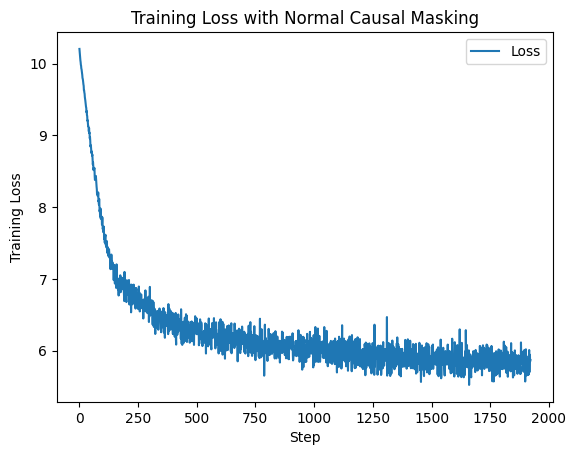
\includegraphics[width=\textwidth]{plots/traininglossnormal.png}
        \caption{Training loss with normal causal masking.}
        \label{fig:traininglossnormal}
    \end{minipage}
    \hfill
    \begin{minipage}[b]{0.45\textwidth}
        \centering
        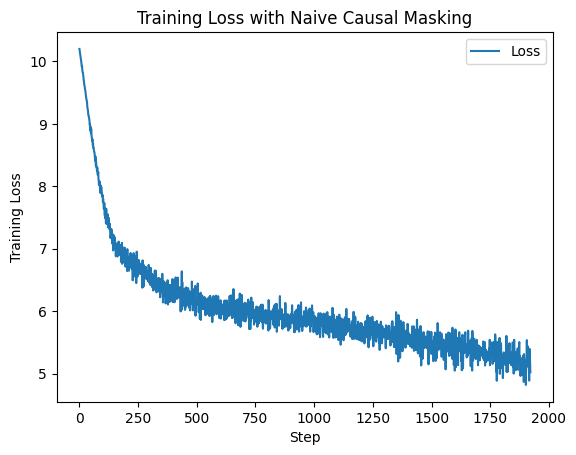
\includegraphics[width=\textwidth]{plots/traininglossnaive.png}
        \caption{Training loss with naive causal masking.}
        \label{fig:traininglossnaive}
    \end{minipage}
\end{figure}

\begin{figure}[htbp]
    \centering
    \begin{minipage}[b]{0.45\textwidth}
        \centering
        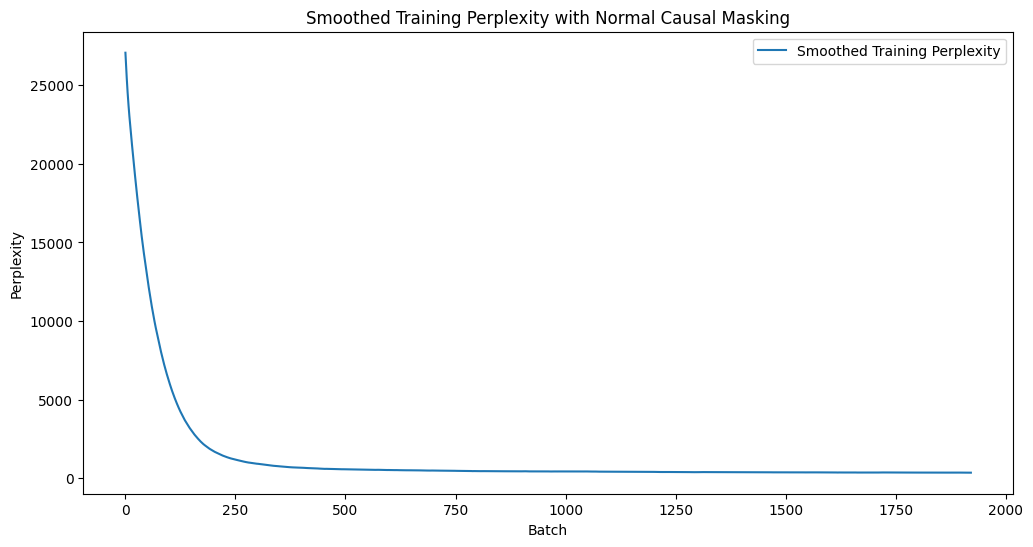
\includegraphics[width=\textwidth]{plots/trainingpplnormal98.png}
        \caption{Smoothed training perplexity with normal causal masking.}
        \label{fig:trainingpplnormal}
    \end{minipage}
    \hfill
    \begin{minipage}[b]{0.45\textwidth}
        \centering
        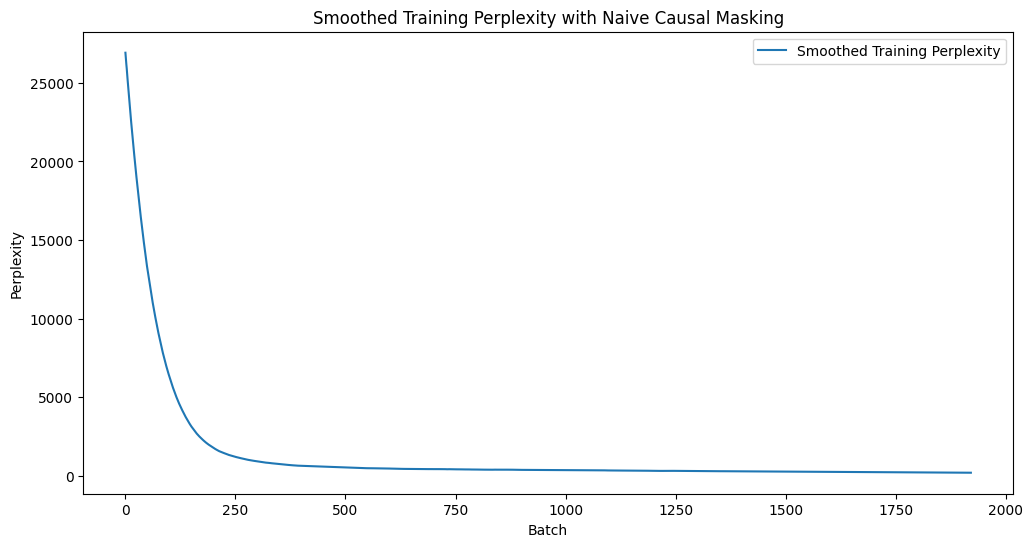
\includegraphics[width=\textwidth]{plots/trainingpplnaive98.png}
        \caption{Smoothed training perplexity with naive causal masking.}
        \label{fig:trainingpplnaive}
    \end{minipage}
\end{figure}

\begin{figure}[htbp]
    \centering
    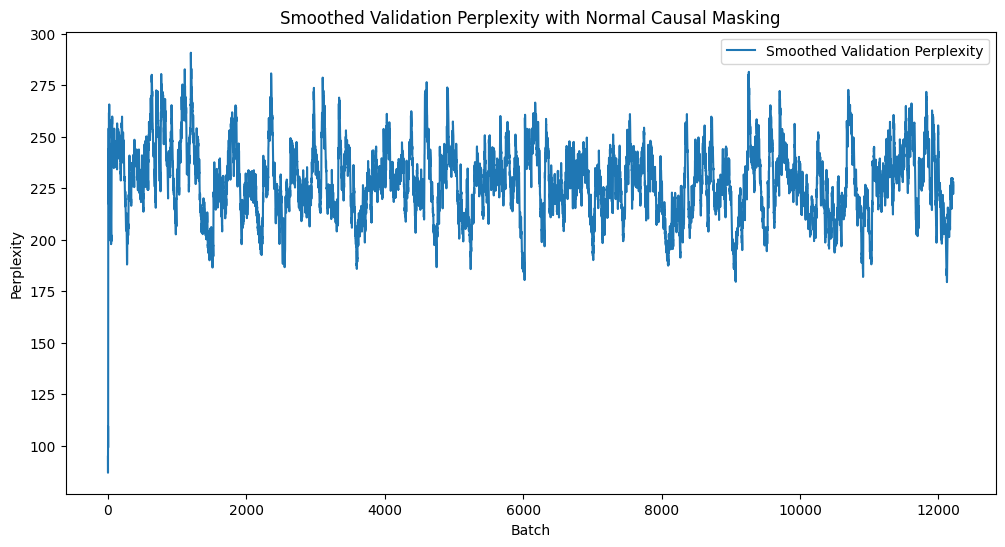
\includegraphics[width=0.8\textwidth]{plots/validationpplnormal98.png}
    \caption{Smoothed validation perplexity with normal causal masking.}
    \label{fig:validationpplnormal}
\end{figure}

\begin{figure}[htbp]
    \centering
    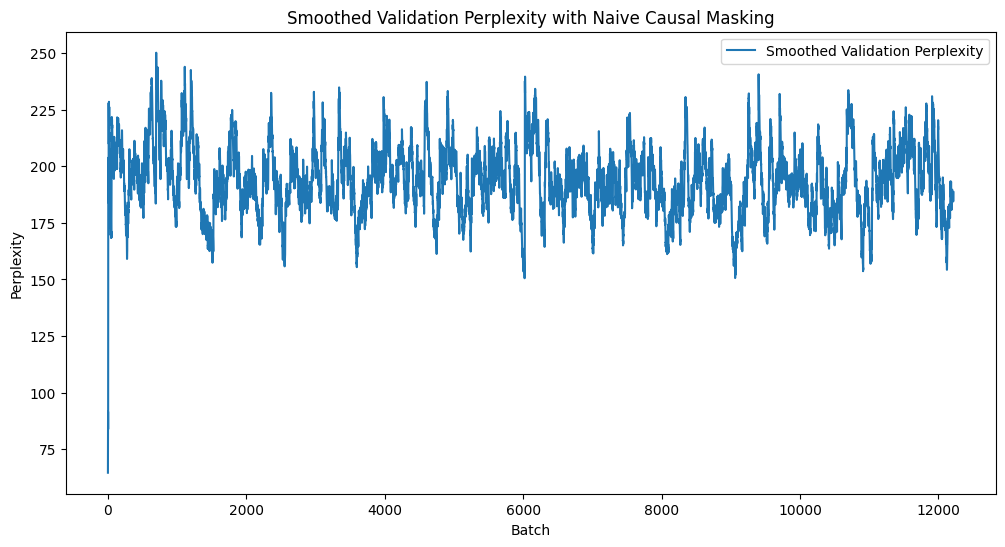
\includegraphics[width=0.8\textwidth]{plots/validationpplnaive98.png}
    \caption{Smoothed validation perplexity with naive causal masking.}
    \label{fig:validationpplnaive}
\end{figure}
\newpage
\begin{table}[htbp]
    \centering
    \begin{tabular}{|c|c|c|}
        \hline
        \textbf{Masking Approach} & \textbf{Training Perplexity} &
        \textbf{Validation Perplexity} \\
        \hline
        Normal Causal Masking & 949.59 & 228.15 \\
        \hline
        Naive Causal Masking & 894.52 & 228.15 \\
        \hline
    \end{tabular}
    \caption{Average Training and Validation Perplexities}
\end{table}

\textbf{Interpretation of results.}

The results were quite interesting! The training loss, training perplexity, and
validation perplexity were all \textit{lower} with naive causal masking than
with normal causal masking. This was quite surprising to me, as I had expected
the naive approach to perform worse than the traditional approach.\\\\
My guess for this is twofold:

\begin{itemize}
    \item The naive approach might have acted as a form of regularization. By
    directly setting the attention scores to 0, regardless of their true value,
    we might have been avoiding overconfidence in certain predictions and ended
    up preventing overfitting to the training data.
    \item The naive approach might have actually worked better than the
    traditional approach, but only on this specific dataset. For example, if the
    dataset has a lot of noise, the traditional approach might be too aggressive
    in masking out future tokens while applying too much probability mass to
    current and past tokens, whereas the naive approach (which could act as a
    regularizer) might actually work better. Then again, I can't be sure of this
    without further experimentation on different datasets.
\end{itemize}

My gut tells me that the naive approach is not as good as the normal approach, I
mean it's literally called the ``naive" approach. But the results are the
results, and I can't argue with them. I would like to do further experimentation
on different datasets to see if the naive approach is actually better than the
normal approach, or if it was just a fluke on this specific dataset. I would
also like to experiment with different hyperparameters and see if the naive
approach is still better than the normal approach, as I just used the same
hyperparameters for both approaches in this experiment.

\newpage

\textbf{Edited code. Plotting functions have been omitted.}
\begin{figure}[htbp]
    \centering
    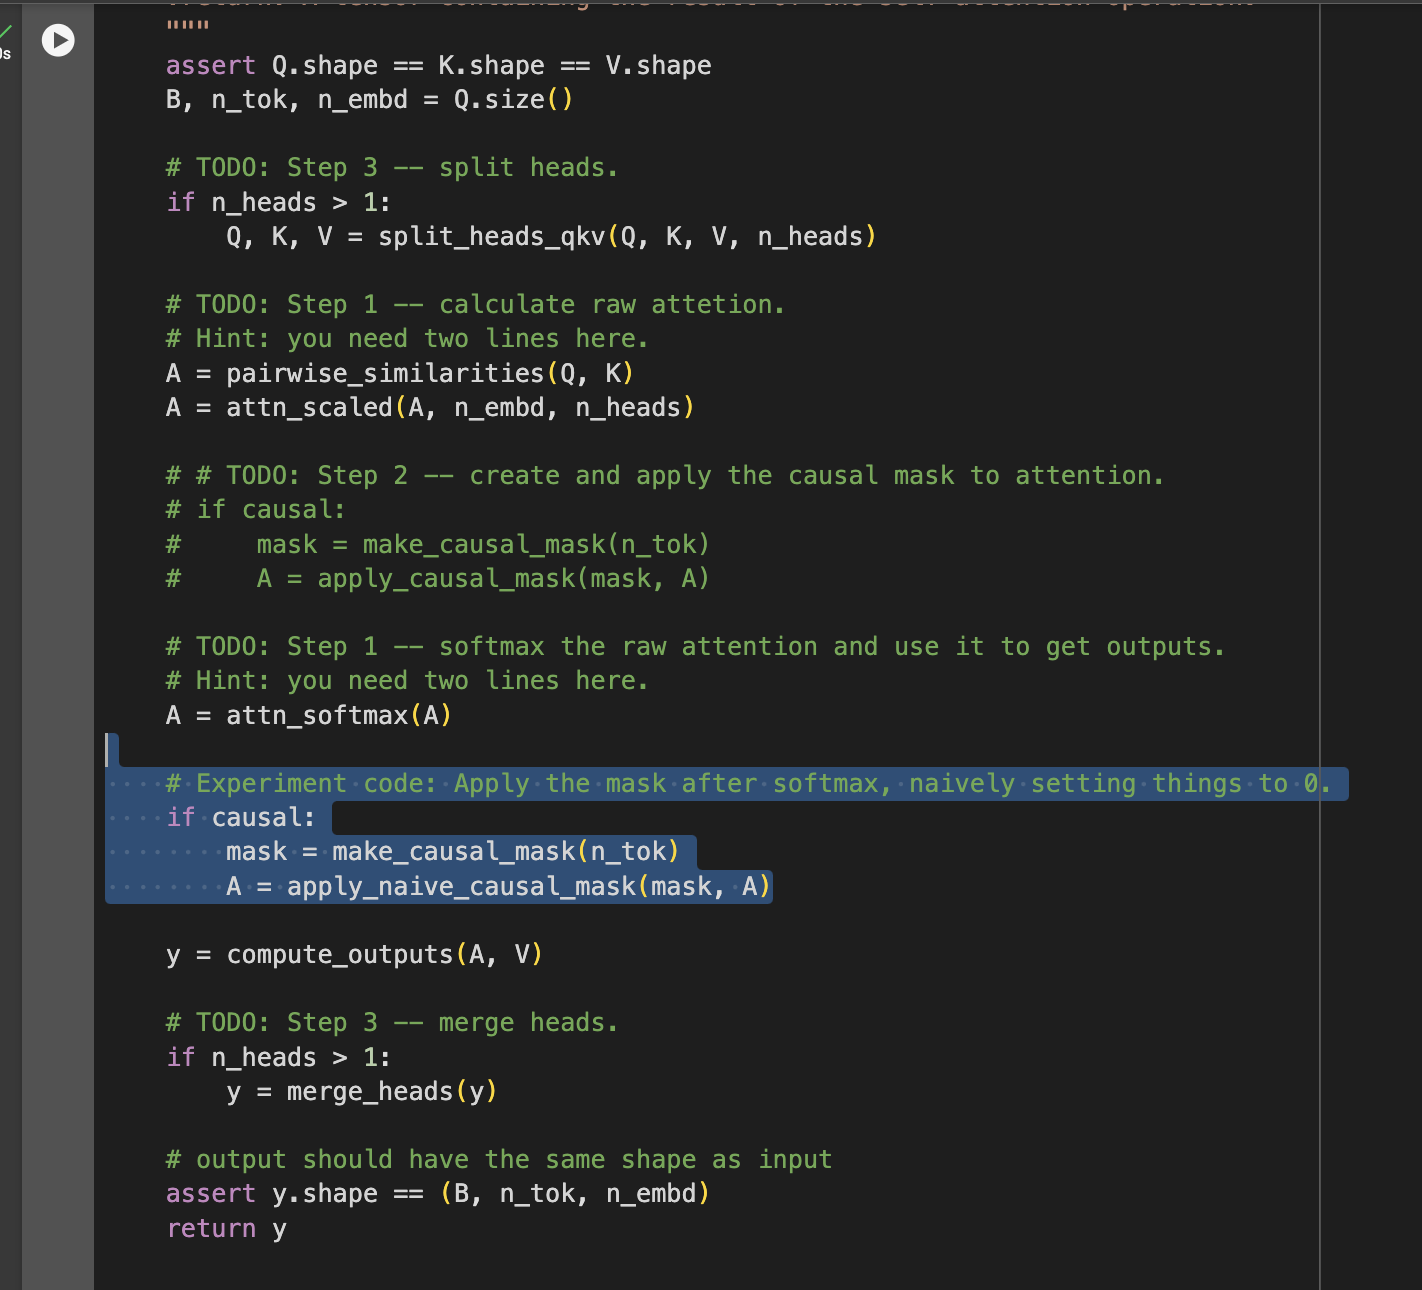
\includegraphics[width=0.8\textwidth]{plots/self_attention.png}
    \caption{The edited code in the self\_attention function. Notice the causal
    masking occurring after the softmax function.}
    \label{fig:selfattention}
\end{figure}

\begin{figure}[htbp]
    \centering
    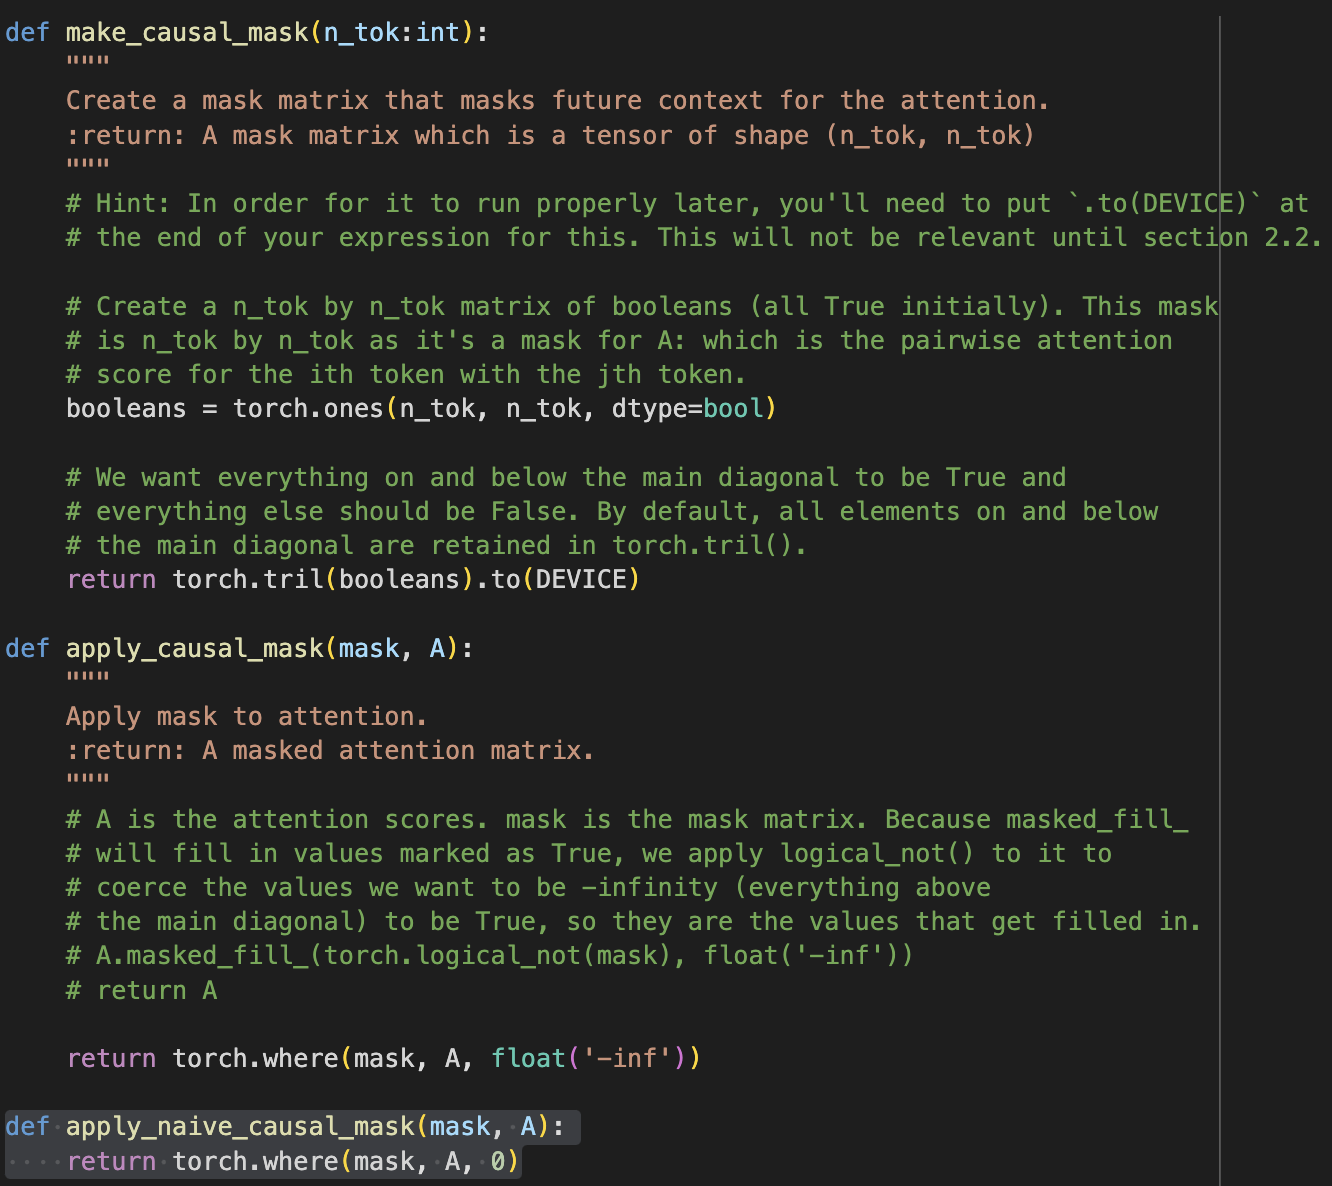
\includegraphics[width=0.8\textwidth]{plots/apply_naive_causal_mask.png}
    \caption{The new naive causal masking function. This was called instead in
    this experiment to compare the regular approach with the naive one.}
    \label{fig:naive_causal_masking}
\end{figure}

\newpage

\section{HuggingFace (40\%)}

In this part of the assignment, you will complete a codebase used to finetune a
pretrained language model (\modelthree) end-to-end on a sentiment analysis task
(\sst) using the convenient infrastructure and tools provided by HuggingFace.
With your implementation, you'll write a short report to answer questions of
your implementation, and analyze the behaviors of your trained model. \textbf{We
will grade both the code and the report.}

\paragraph{Notebook:}
You will use the following Python notebook for this exercise:
\textcolor{blue}{\href{https://colab.research.google.com/drive/13oBf6_e6xc9W9uJIxjndX1z-SwPRysRw?usp=sharing}{A2S3.ipynb}}.

\paragraph{Deliverables:} 

\begin{enumerate}
\item \textbf{Coding Exercises:} You should complete the code blocks denoted by
\texttt{TODO:} in the Python notebook. To submit your code, download your
notebook as a Python file (\verb|A2S3.py|).
\item \textbf{Write-up:} Your report for this part should be \textbf{no more
than four pages}, and should answer all questions listed in \S 3.2. 
\end{enumerate}

\subsection{Background}

The pretrain-then-finetune pipeline is a common recipe for large language model
(LLM) applications and research. Essentially, the \textit{pretraining} step
leverages the vast amount of raw data gathered through the internet to train a
model in an unsupervised way to capture the underlying knowledge patterns and
structure of language. Next, the \textit{finetuning} step customizes pretrained
models to specific applications and tasks, building on top of their existing
capabilities. In this exercise, you will complete a codebase that is used to
finetune a \texttt{\modelthree} model on a sentiment analysis task (\sst) using
the HuggingFace library. 

\paragraph{Pretrained Model}

\texttt{RoBERTa} is a Transformers-based bidirectional encoder-only language
model pretrained with masked language modeling objective\footnote{The
\texttt{RoBERTa} paper: \url{https://arxiv.org/abs/1907.11692}}. Encoder-only
models like \texttt{RoBERTa} are useful for encoding input sequences for
classification tasks, rather than open-ended text generation. In this exercise,
you will finetune a pretrained \texttt{\modelthree} model that is already
provided for you by HuggingFace.

\paragraph{Dataset/Task}
The Stanford Sentiment Treebank (\sst) is a corpus labeled for the
sentence-level sentiment analysis task, consisting of 11,855 single sentences
extracted from movie reviews.\footnote{See details of SST-2 at
\url{https://huggingface.co/datasets/sst2}.} Each data point in the dataset
consists of an input sentence and an output sentiment label (1 for positive and
0 for negative).

\subsection{Finetuning Your Own \texttt{RoBERTa} Classifier}

The provided Python notebook breaks the task down into the following six steps:

\begin{itemize}
    \item Step 0: Preperation
    \item Step 1: Defining PyTorch Dataset and Dataloader
    \item Step 2: Load Data
    \item Step 3: Training and Evaluation
    \item Step 4: Main Training Loop
    \item Step 5: Testing the Final Model
\end{itemize}

\paragraph{For each of Step 1-5, you will complete the following two tasks:}

\begin{enumerate}
    \item \textbf{Coding Exercises} in the \textbf{notebook}: You will complete
    the the code blocks denoted by \texttt{TODO:}.
    \item \textbf{Questions to Answer} in the \textbf{report/write-up}: You will
    answer questions denoted by \texttt{Q:}.
\end{enumerate}

For the full context of this exercise, please refer to the notebook. You should
be able to answer the questions once you finish implementing the code blocks. As
the \textbf{Coding Exercises} and \textbf{Questions to Answer} are interleaving
and interdependent, \textbf{Questions to Answer} are best understood in
conjunction with \textbf{Coding Exercises} in the notebook. However, to
streamline your report/write-up, we list the questions below as a checklist for
your report.

\begin{itemize}
    \item[\textit{Step 1:}] \textit{Defining PyTorch Dataset and Dataloader}
    
    \begin{itemize}
        \item[\textbf{Q1.1:}] \textbf{Explain the usages of the following
        arguments when you encode the input texts: \texttt{padding},
        \texttt{max\_length}, \texttt{truncation}, \texttt{return\_tensors}.}
        
        \begin{itemize}
            \item \texttt{padding} --- When batching sequences together, each
            sequence needs to be the same length. Padding is applied to make
            sure all sequences in a batch are the same length for the model to
            process them in parallel. If \texttt{padding = True | "longest"},
            the tokenizer will add a special token to the sequences shorter than
            the longest sequence in the batch to match its length.

            \item \texttt{truncation} --- If \texttt{truncation = True},
            sequences longer than \texttt{max\_length} will be truncated down to
            that length. 

            \item \texttt{max\_length} --- This is the maximum length of the
            sequence after tokenization. If a sequence is longer than
            \texttt{max\_length}, it will be truncated to this length.

            \item \texttt{return\_tensors} --- Setting \texttt{return\_tensors =
            "pt"} tells the tokenizer to return the sequences as PyTorch
            tensors. Other options include \texttt{"tf"} for TensorFlow tensors
            or \texttt{"np"} for NumPy arrays.
        \end{itemize}

        \texttt{https://huggingface.co/docs/transformers/v4.37.2/en/main\_classes\\
        /tokenizer\#transformers.PreTrainedTokenizerFast.encode} was very
        helpful for understanding these arguments.

        \item[\textbf{Q1.2:}] \textbf{For the above arguments, explain what are
        the potential advantages of setting them to the default values we
        provide.}

        \begin{itemize}
            \item \texttt{padding=True} --- We're ensuring that all sequences in
            a batch have the same length. This uniformity is required for batch
            processing on GPUs, which significantly speeds up training and
            evaluation since matrix operations on a GPU are highly parallelized.
            Without padding, batch processing would not be possible, and each
            sequence would need to be processed individually, which is way more
            inefficient.

            \item \texttt{truncation=True} --- By enabling truncation, we're
            making sure that any sequence longer than 512 tokens is cut down,
            preventing errors from sequences that are too long for the model to
            handle.

            \item \texttt{max\_length=512} --- I looked it up, and it seems like
            many transformer models (like BERT) are trained on a maximum
            sequence length of 512 tokens. I guess this ensures we're using the
            model in the way it was designed and trained for, and also manages
            memory usage by keeping the sequences bounded.

            \item \texttt{return\_tensors="pt"} --- We can feed the sequences
            directly into the model without any further processing, since
            they're already in PyTorch tensor format. This is convenient and
            saves time and memory.
        \end{itemize}
    \end{itemize}

    \item[\textit{Step 2:}] \textit{Loading Data}
    
    \begin{itemize}
        \item[\textbf{Q2.1:}] \textbf{What are the lengths of train, validation,
        test datasets?}

        \begin{itemize}
            \item \textbf{Training set}: 6,920
            \item \textbf{Validation set}: 872
            \item \textbf{Test set}: 1,821
        \end{itemize}
        
        \item[\textbf{Q2.2:}] \textbf{Explain the role of each of the following
        parameters: \texttt{batch\_size}, \texttt{shuffle},
        \texttt{collate\_fn}, \texttt{num\_workers} given to the
        \texttt{DataLoader} in the above code block.}

        \begin{itemize}
            \item \texttt{batch\_size} --- The number of samples we want to pass
            into the training loop at each iteration.
            \item \texttt{shuffle} --- Set to \texttt{True} if we want to
            shuffle the data at every epoch.
            \item \texttt{collate\_fn} --- The function used to collate the
            samples into a batch. In this case, we are passing
            \texttt{SST2Dataset.collate\_fn} as our function, which does the
            tokenization and returns a dictionary of tensors for the input
            sequences and the labels.
            \item \texttt{num\_workers} --- The number of parallel subprocesses
            we want to use when we're loading all data. This just speeds up the
            data loading process.
        \end{itemize}
        
        \item[\textbf{Q2.3:}] \textbf{Write the \textbf{type} and \textbf{shape}
        (if the type is tensor) of \texttt{input\_ids},
        \texttt{attention\_mask}, and \texttt{label\_encoding} in \texttt{batch}
        and explain \textbf{what these elements represent}.}

        All are tensors. Note that the batch size equals 64 and the sequence
        length equals 45.

        \begin{itemize}
            \item \texttt{input\_ids} (shape: \texttt{[64, 45]}) --- Each number
            in \texttt{input\_ids} is a token ID that corresponds to a
            particular token in the tokenizer's vocabulary. The model uses these
            IDs to look up the embedding for each token and process the input
            sequence.
            \item \texttt{attention\_mask} (shape: \texttt{[64, 45]}) --- The
            attention mask designates which tokens are actual tokens versus
            padding tokens in \texttt{input\_ids}. A value of 1 indicates a real
            token, and 0 indicates a padding token. This mask makes sure that
            the model does not attend to padding positions when processing the
            input.
            \item \texttt{label\_encoding} (shape: \texttt{[64]}) --- This is
            the label for each sequence in the batch. A value of 1 indicates a
            positive sentiment, and 0 indicates a negative sentiment. These are
            like the truth values we're trying to predict, which the model will
            compare against its predictions to calculate the loss during
            training.
        \end{itemize}

    \end{itemize}
    
    \item[\textit{Step 3:}] \textit{Training and Evaluation}

    \begin{itemize}
        \item[\textbf{Q3.1:}] \textbf{For the three lines of code you
        implemented for computing gradients and updating parameters using
        optimizer, explain what each of the lines does, respectively.}

        \begin{enumerate}
            \item \texttt{optimizer.zero\_grad()} --- This line clears the
            gradients from the previous batch. This is because in PyTorch,
            gradients are accumulated by default, so we need to clear them
            because otherwise our gradients would mix across batches.

            \item \texttt{loss.backward()} --- This line computes the gradient
            of the loss with respect to all the parameters in the model
            (technically, all the parameters that have
            \texttt{requires\_grad=True}). This is just backpropagation.

            \item \texttt{optimizer.step()} --- This line actually performs the
            update based on the gradients we just computed in the last line. We
            update the parameters by taking a step in the direction of the
            negative gradient, scaled by the learning rate (direction of
            steepest descent).
        \end{enumerate}
        
        \item[\textbf{Q3.2:}] \textbf{Explain what setting the model to training
        and evaluation modes do, respectively.}
        
        It turns out there are some layers like \texttt{Dropout} and
        \texttt{BatchNorm} that are used during training but not during
        evaluation. For example, \texttt{Dropout} randomly zeroes some of the
        input tensor elements with a probability of $p$ at each step during
        training which apparently is effective for regularization. Batch
        normalization uses batch statistics to normalize the input tensor, which
        is also different between training and evaluation. So, setting the model
        to training mode turns on these layers, and setting the model to
        evaluation mode turns them off. Evaluation mode means the model behaves
        more consistently, and we can use it to make predictions on new data.
        
        \item[\textbf{Q3.3:}] \textbf{Explain what \texttt{with
        torch.no\_grad()} does in the \texttt{evaluation()} function.}

        We don't need to compute gradients during evaluation because we're not
        updating the model's parameters. Thus, if we want to save memory and
        compute time, we can disable gradient computation, which is what
        \texttt{torch.no\_grad()} does. It's specifically a context manager,
        which allows the code inside the block to run without gradient
        computation.

        Read more: \texttt{https://realpython.com/python-with-statement/}

    \end{itemize}

    \item[\textit{Step 4:}] \textit{Main Training Loop}

    \begin{itemize}
        \item[\textbf{Q4.1:}] \textbf{With the following default hyperparameters
        we provide, plot both training and validation loss curves across 10
        epochs in a single plot ($x$-axis: num of the epoch; $y$-axis: acc). You
        can draw this plot with a Python script or other visualization tools
        like Google Sheets. (\texttt{batch\_size = 64}, \texttt{learning\_rate =
        5e-5}, \texttt{num\_epochs = 20}, \texttt{model\_name =
        "roberta-base"})}

        \begin{figure}[h]
            \centering
            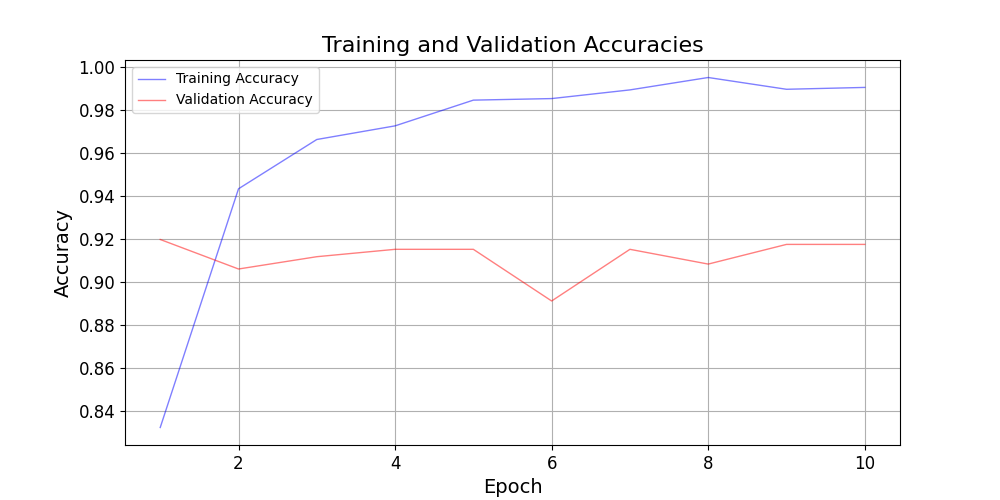
\includegraphics[width=\textwidth]{plots/adamw.png}
            \caption{Training and validation accuracies across 10 epochs with
            optimizer \texttt{AdamW}, $\eta = 5 \cdot 10^{-5}$, and $\varepsilon
            = 1 \cdot 10^{-8}$.}
        \end{figure}
        
        
        \item[\textbf{Q4.2:}] \textbf{Describe the behaviors of the training and
        validation loss curves you plotted above. At which epoch does the model
        achieve the best accuracy on the training dataset? What about the
        validation dataset? Do training and validation curves have the same
        trend? Why does the current trend happen?}

        The training accuracy starts off low and increases rapidly, while the
        validation accuracy starts off high and doesn't really change much. The
        model achieves the best accuracy on the training dataset in the
        3rd-to-last epoch, however, the training accuracy in the last 3 epochs
        was almost at 1.0 anyways.

        The validation accuracy surprisingly was highest in the first epoch, and
        it even decreased after that (although not by much).

        The training and validation curves don't have the same trend. The
        training accuracy increases rapidly, while the validation accuracy
        doesn't really change much. This is likely because the model is
        overfitting to the training data, which is why the training accuracy
        keeps increasing while the validation accuracy doesn't. The model is
        learning the training data too well, and it's not generalizing well to
        the validation data.
        
        \item[\textbf{Q4.3:}] \textbf{Why do you shuffle the training data but
        not the validation data?}

        We shuffle the training data because we want to randomize the order of
        the training samples at the beginning of each epoch. This is important
        because we want the model to learn to generalize well to the entire
        training dataset, not just the order of the samples.

        We don't shuffle the validation data because we don't need to. We're not
        updating the model's parameters during validation, so the order of the
        samples doesn't matter.
        
        \item[\textbf{Q4.4:}] \textbf{Explain the functionality of optimizers.}
        
        Optimizers are algorithms that are used to update the parameters of the
        model based on the gradients of the loss function. They are used to
        minimize the loss function by computing its gradient with respect to the
        model's parameters and updating the parameters in the direction of the
        negative gradient, scaled by the learning rate. This allows the
        parameters to flow towards the minimum of the loss function, which is
        where the model is most accurate.
        
        \item[\textbf{Q4.5:}] \textbf{Experiment with two other optimizers
        defined in \texttt{torch.optim} for the training the model with the
        default hyperparameters we give you. What is the difference between
        \texttt{AdamW} and these two new optimizers? Back up your claims with
        empirical evidence.}

        I experimented with \texttt{SGD} and \texttt{Adagrad}.

        \begin{itemize}
            \item \texttt{SGD} --- The training accuracy and evaluation accuracy
            is much lower than with \texttt{AdamW}. It started out near 50\% for
            both and didn't really change much! The model is not learning as
            well with \texttt{SGD} as it is with \texttt{AdamW}. I did not
            bother to plot the training and validation accuracies across 10
            epochs with \texttt{SGD} because it was bad and didn't change much.

            \item \texttt{Adagrad} --- With \texttt{Adagrad}, the training and
            validation accuracy were actually \textit{higher} than with
            \texttt{AdamW}. The training accuracy started out above 87\% and
            climbed to 98\% by the end, while the validation accuracy started
            out at 91\% or so and even got to 93\% by the end!
        \end{itemize}
        \begin{figure}[h]
            \centering
            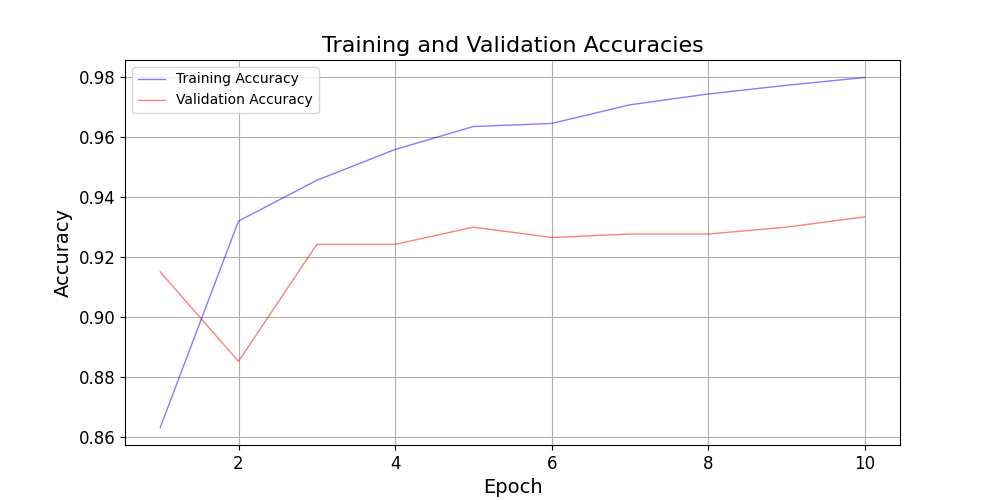
\includegraphics[width=\textwidth]{plots/adagrad.png}
            \caption{Training and validation accuracies across 10 epochs with
            optimizer \texttt{Adagrad}, $\eta = 5 \cdot 10^{-5}$, and
            $\varepsilon = 1 \cdot 10^{-8}$.}
        \end{figure}
        
        \item[\textbf{Q4.6:}] \textbf{Experiment with different combinations of
        \texttt{batch\_size}, \texttt{learning\_rate}, and \texttt{num\_epochs}.
        Your goal is to pick the final, best model checkpoint based on the
        validation dataset accuracy. Describe the strategy you used to try
        different combinations of hyperparameters. Why did you use this
        strategy?}

        I tried different combinations of \texttt{batch\_size},
        \texttt{learning\_rate}, and \texttt{num\_epochs} by using a grid
        search. I tried a few different values for each hyperparameter and
        trained the model with each combination. I then picked the combination
        that gave the highest validation accuracy.

        I used this strategy because it's a simple and systematic way to try
        different combinations of hyperparameters. I wanted to make sure I
        didn't miss any good combination. A grid search is a good way to do this
        because it's easy to implement and it's easy to understand.
        
        \item[\textbf{Q4.7:}] \textbf{What are the \texttt{batch\_size},
        \texttt{learning\_rate}, and \texttt{num\_epochs} of the best model
        checkpoint that you picked? What are the training accuracy and
        validation accuracy?}

        The best configuration of hyperparameters I found was:
        \begin{itemize}
            \item \texttt{batch\_size} = 64
            \item \texttt{learning\_rate} = $2 \cdot 10^{-6}$
            \item \texttt{num\_epochs} = 10
        \end{itemize}

    \end{itemize}

    \item[\textit{Step 5:}] \textit{Testing the Final Model}
    \begin{itemize}
        \item[\textbf{Q5.1:}] \textbf{What's the test set accuracy of the best
        model?}

        The test set accuracy I got on my best model was
        $\boxed{0.9330038440417353}$.
    \end{itemize}
    
\end{itemize}


\end{document}
% \theend
